\documentclass[preview,border=0mm,convert={density=600,outext=.png}]{standalone}
\usepackage{amsfonts,amssymb,amsmath}
\usepackage{tikz}
\usetikzlibrary{automata,shapes,patterns,calc,arrows}
\usepackage{xspace}
\usetikzlibrary{arrows}
\usetikzlibrary{automata}
\usetikzlibrary{shapes,snakes}
\usetikzlibrary{calc}
\usetikzlibrary{patterns}
\usetikzlibrary{shapes.geometric}
\usetikzlibrary{positioning}
\tikzstyle{action}=[rounded corners=.5,minimum size=.4cm,draw=gray!90,inner sep=1pt,fill=gray!20,very thick]
\tikzstyle{every edge}=[draw,>=stealth',shorten >=1pt]

%\tikzset{node distance=2.5cm}
%\tikzset{every node/.style={anchor=base}}

%% edges
\tikzset{>=latex,bend angle=20}
\tikzstyle{line}=[line width=.6pt]
\tikzstyle{arrow}=[->,line]
\tikzstyle{dblarrow}=[<->,line]
\tikzstyle{invarrow}=[<-,line]
\tikzstyle{initial}=[invarrow]
\tikzset{selfloop/.style={arrow,out={#1-30},in={#1+30},looseness=6}}
% we use tikzset here because tikzstyle does not allow arguments
 

\begin{document}

\centering
  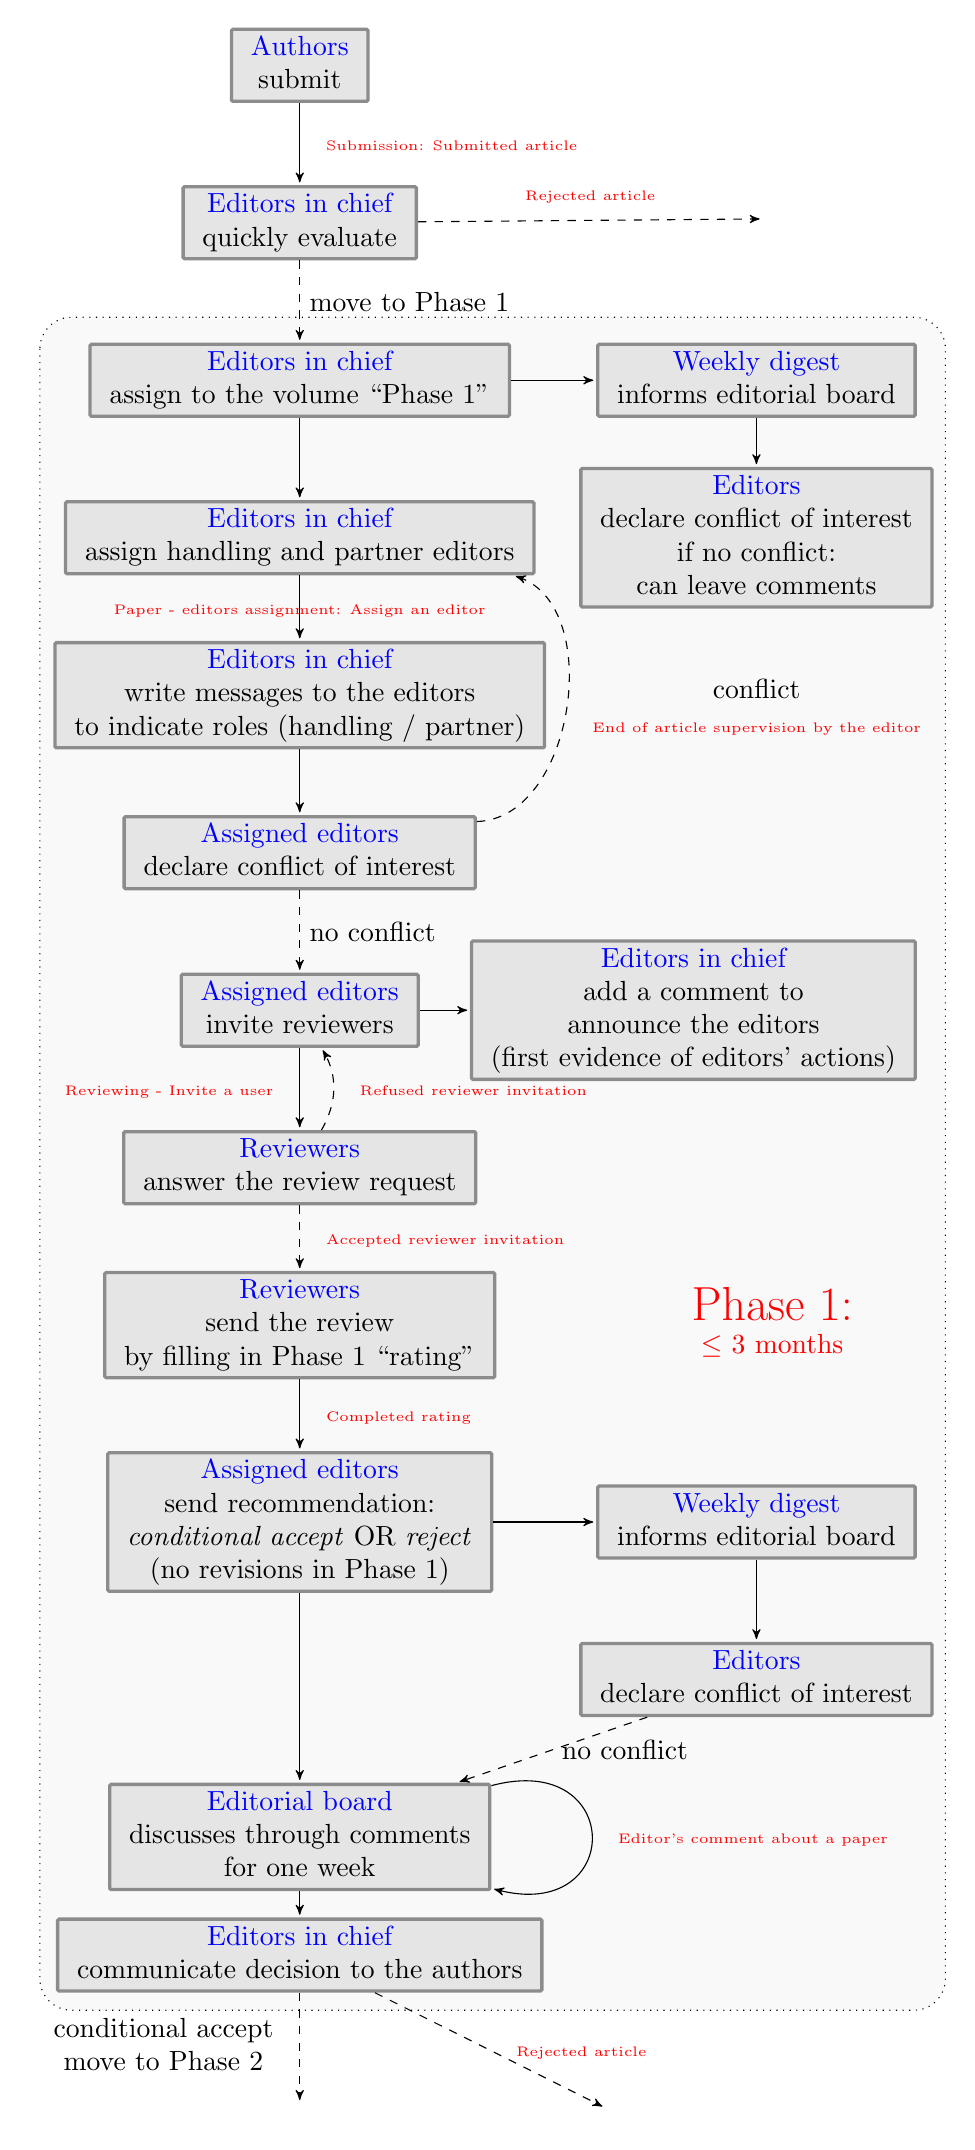
\begin{tikzpicture}


    \draw[dotted,rounded corners=4mm,fill=gray!5]
    ($(-3.3,-3.2)$) rectangle ($(8.2,-24.7)$) ;

    \node[action] (submit) at (0,0) {\begin{tabular}{c}\textcolor{blue}{Authors}\\ submit\end{tabular}};
    \node[action] (quickevaluate) at (0,-2) {\begin{tabular}{c}\textcolor{blue}{Editors in chief}\\ quickly evaluate\end{tabular}};
    \node (reject1) at (6,-1.95) {\ };
    \node[action] (assignvolume1) at (0,-4) {\begin{tabular}{c}\textcolor{blue}{Editors in chief}\\ assign to the volume ``Phase 1''\end{tabular}};
    \node[action] (weeklydigest) at (5.8,-4) {\begin{tabular}{c}\textcolor{blue}{Weekly digest}\\ informs editorial board\end{tabular}};
    \node[action] (assigneditors) at (0,-6) {\begin{tabular}{c}\textcolor{blue}{Editors in chief}\\ assign handling and partner editors\end{tabular}};
    \node[action] (registerinterest) at (5.8,-6) {\begin{tabular}{c}\textcolor{blue}{Editors}\\ declare conflict of interest\\ if no conflict:\\ can leave comments\end{tabular}};
    \node[action] (indicateroles) at (0,-8) {\begin{tabular}{c}\textcolor{blue}{Editors in chief}\\ write messages to the editors \\ to indicate roles (handling / partner)\end{tabular}};
    \node[action] (declarecoi) at (0,-10) {\begin{tabular}{c}\textcolor{blue}{Assigned editors}\\ declare conflict of interest\end{tabular}};
    \node[action] (invitereviewers) at (0,-12) {\begin{tabular}{c}\textcolor{blue}{Assigned editors}\\ invite reviewers\end{tabular}};
    \node[action] (announceeditors) at (5,-12) {\begin{tabular}{c}\textcolor{blue}{Editors in chief}\\ add a comment to \\ announce the editors\\ (first evidence of editors' actions)\end{tabular}};
    \node[action] (answerreview) at (0,-14) {\begin{tabular}{c}\textcolor{blue}{Reviewers}\\ answer the review request \end{tabular}};
    \node[action] (sendreview) at (0,-16) {\begin{tabular}{c}\textcolor{blue}{Reviewers}\\ send the review \\ by filling in Phase 1 ``rating''\end{tabular}};
    \node[action] (recommendation) at (0,-18.5) {\begin{tabular}{c}\textcolor{blue}{Assigned editors}\\ send recommendation:\\ \textit{conditional accept} OR \textit{reject}\\ (no revisions in Phase 1)\end{tabular}};
    \node[action] (weeklydigest2) at (5.8,-18.5) {\begin{tabular}{c}\textcolor{blue}{Weekly digest}\\ informs editorial board\end{tabular}};
    \node[action] (registerinterest2) at (5.8,-20.5) {\begin{tabular}{c}\textcolor{blue}{Editors}\\ declare conflict of interest\end{tabular}};
    \node[action] (decide) at (0,-22.5) {\begin{tabular}{c}\textcolor{blue}{Editorial board}\\ discusses through comments\\ for one week\end{tabular}};
    \node[action] (communicatedecision) at (0,-24) {\begin{tabular}{c}\textcolor{blue}{Editors in chief}\\ communicate decision to the authors\end{tabular}};
    \node (phase2) at (0,-26) {\ };
    \node (reject2) at (4,-26) {\ };

    \node (unnamed) at (6,-16) {\begin{tabular}{c}\textcolor{red}{\LARGE{Phase 1:}}\\ \textcolor{red}{$\le$ 3 months}\end{tabular}};
  
    \draw[->] (submit) edge node[right] {\begin{tabular}{c}\tiny{\color{red} Submission: Submitted article}\end{tabular}} (quickevaluate) ;
    \draw[dashed, ->] (quickevaluate) edge node[above] {\begin{tabular}{c}\tiny{\color{red} Rejected article}\end{tabular}} (reject1) ;
    \draw[dashed, ->] (quickevaluate) edge node[right] {move to Phase 1} (assignvolume1) ;
    \draw[->] (assignvolume1) edge (assigneditors) ;
    \draw[->] (assignvolume1) edge (weeklydigest) ;
    \draw[->] (assigneditors) edge node {\begin{tabular}{c}\tiny{\color{red} Paper - editors assignment: Assign an editor}\end{tabular}} (indicateroles) ;
    \draw[->] (indicateroles) edge (declarecoi) ;
    \draw[->] (weeklydigest) edge (registerinterest) ;
    \draw[dashed, ->] (declarecoi) edge node[right] {no conflict} (invitereviewers) ;
    \draw[dashed, ->] (declarecoi) edge[bend right=80] node[right] {\begin{tabular}{c}conflict\\ \tiny{\color{red} End of article supervision by the editor}\end{tabular}} (assigneditors) ;
    \draw[->] (invitereviewers) edge (announceeditors) ;
    \draw[->] (invitereviewers) edge node[left] {\begin{tabular}{c}\tiny{\color{red} Reviewing - Invite a user}\end{tabular}} (answerreview) ;
    \draw[dashed, ->] (answerreview) edge node[right] {\begin{tabular}{c}\tiny{\color{red} Accepted reviewer invitation}\end{tabular}} (sendreview) ;
    \draw[dashed, ->] (answerreview) edge[bend right=30] node[right] {\begin{tabular}{c}\tiny{\color{red} Refused reviewer invitation}\end{tabular}} (invitereviewers) ;
    \draw[->] (sendreview) edge node[right] {\begin{tabular}{c}\tiny{\color{red} Completed rating}\end{tabular}} (recommendation) ;
    \draw[dashed, ->] (registerinterest2) edge node[right] {no conflict} (decide) ;
    \draw[->] (recommendation) edge (weeklydigest2) ;
    \draw[->] (weeklydigest2) edge (registerinterest2) ;
    \draw[->] (recommendation) edge (decide) ;
    \draw[->] (decide) edge [distance = 50, in = 0, out = 0, loop right] node[right] {\begin{tabular}{c}\tiny{\color{red} Editor's comment about a paper}\end{tabular}} (decide) ;
    \draw[->] (decide) edge (communicatedecision) ;
    \draw[dashed, ->] (communicatedecision) edge node[right] {\begin{tabular}{c}\tiny{\color{red} Rejected article}\end{tabular}} (reject2) ;
    \draw[dashed, ->] (communicatedecision) edge node[left] {\begin{tabular}{c}conditional accept\\ move to Phase 2\end{tabular}} (phase2) ;
  \end{tikzpicture}

\end{document}